\begin{frame}
\frametitle{Similar feature spaces}

\centering
\begin{tikzpicture}
\uncover<1>{\node{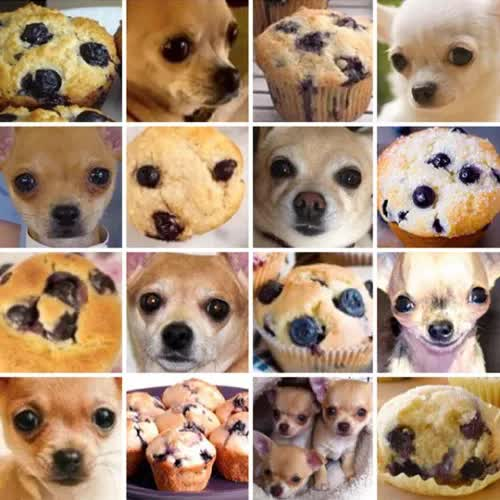
\includegraphics[height=3.0in]{img/dog-or-food1}};}
\uncover<2>{\node{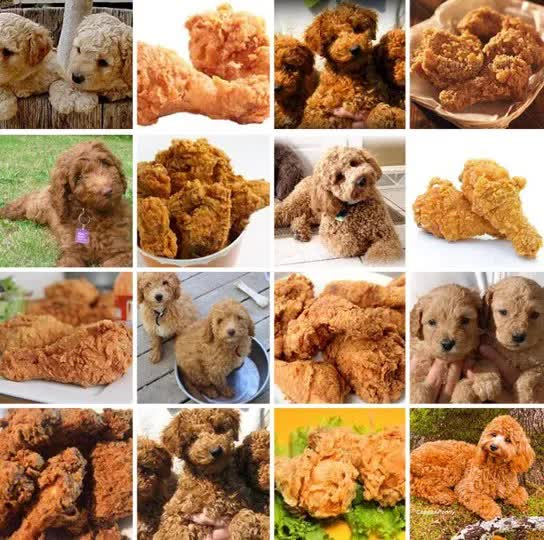
\includegraphics[height=3.0in]{img/dog-or-food2}};}
\uncover<3>{\node{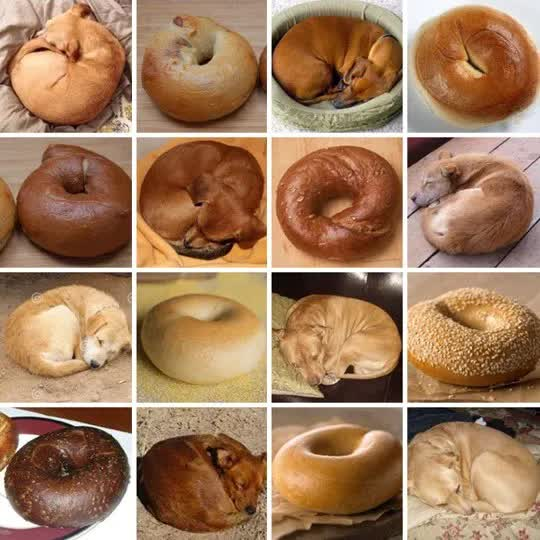
\includegraphics[height=3.0in]{img/dog-or-food3}};}
\uncover<4>{\node{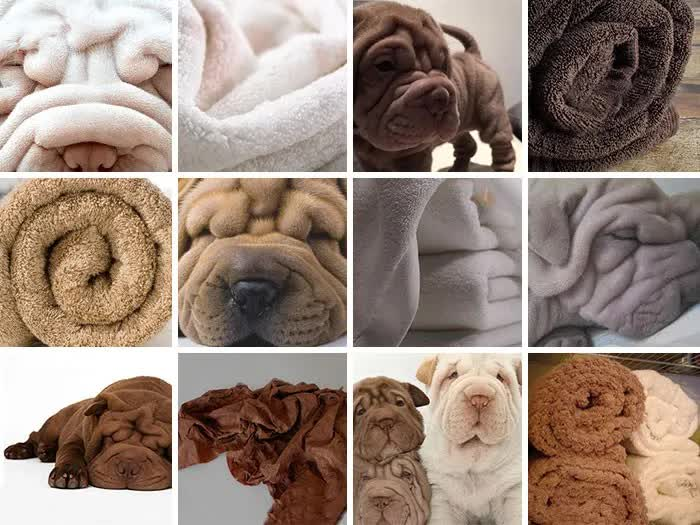
\includegraphics[height=3.0in]{img/dog-or-food4}};}
\uncover<5>{\node{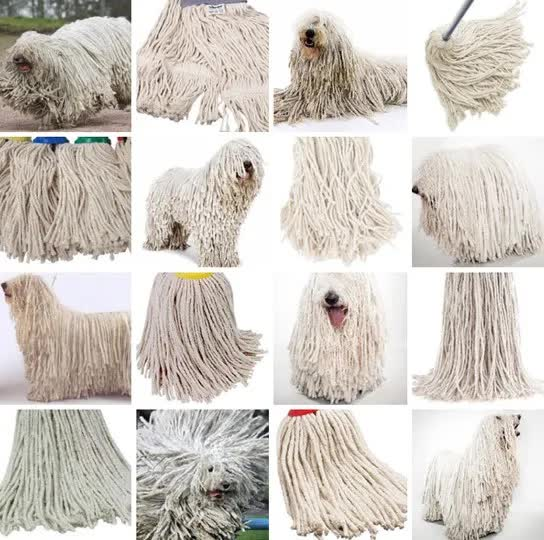
\includegraphics[height=3.0in]{img/dog-or-food5}};}
\uncover<6>{\node{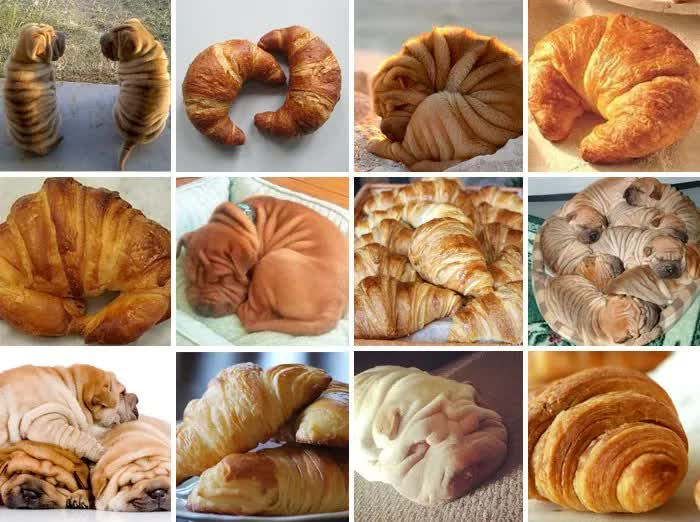
\includegraphics[height=3.0in]{img/dog-or-food6}};}
\uncover<7>{\node{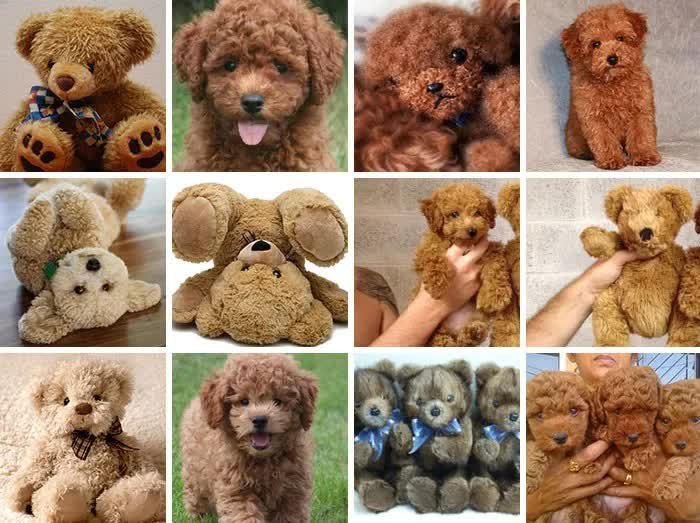
\includegraphics[height=3.0in]{img/dog-or-food7}};}
\end{tikzpicture}

%{
%\tiny
%\url{https://neurabites.com/muffin-or-chihuahua/}
%}
%
%These images are similar in \textbf{feature space} but not \textbf{class semantics}.
%
%We are interested only in \textbf{class semantics}.
\end{frame}
